\documentclass{article}
\usepackage{graphicx} % Required for inserting images
\usepackage{amsmath, amssymb, mathtools}
\usepackage{dirtytalk}
\graphicspath{{Images/}}

\setlength{\oddsidemargin}{0in}
\setlength{\textwidth}{6.5in}
\setlength{\topmargin}{-.55in}
\setlength{\textheight}{9in}
\pagestyle{empty}


\title{Optimization HW 3}
\author{Michael Nameika}
\date{}

\begin{document}

\maketitle

\section*{Section 4.1 Problems}
\textbf{1.} Solve the following linear programs graphically.
\begin{itemize} 
    \item[(ii)] 
    \begin{align*}
       \:\:\: \text{maximize} \:\:\: z = x_1 + 2&x_2 \\
        \text{subject to} \:\:\:\: 2x_1 + x_2 &\geq 12\\
        x_1 + x_2 &\geq 5 \\
        -x_1 + 3x_2 &\leq 3\\
        6x_1 - x_2 &\geq 12\\
        x_1,x_2 &\geq 0.
    \end{align*}
    Notice from the below plot that the feasible region is unbounded, and that $z$ increases in the direction of unboundedness, so this problem has no maximum.
    \begin{center}
        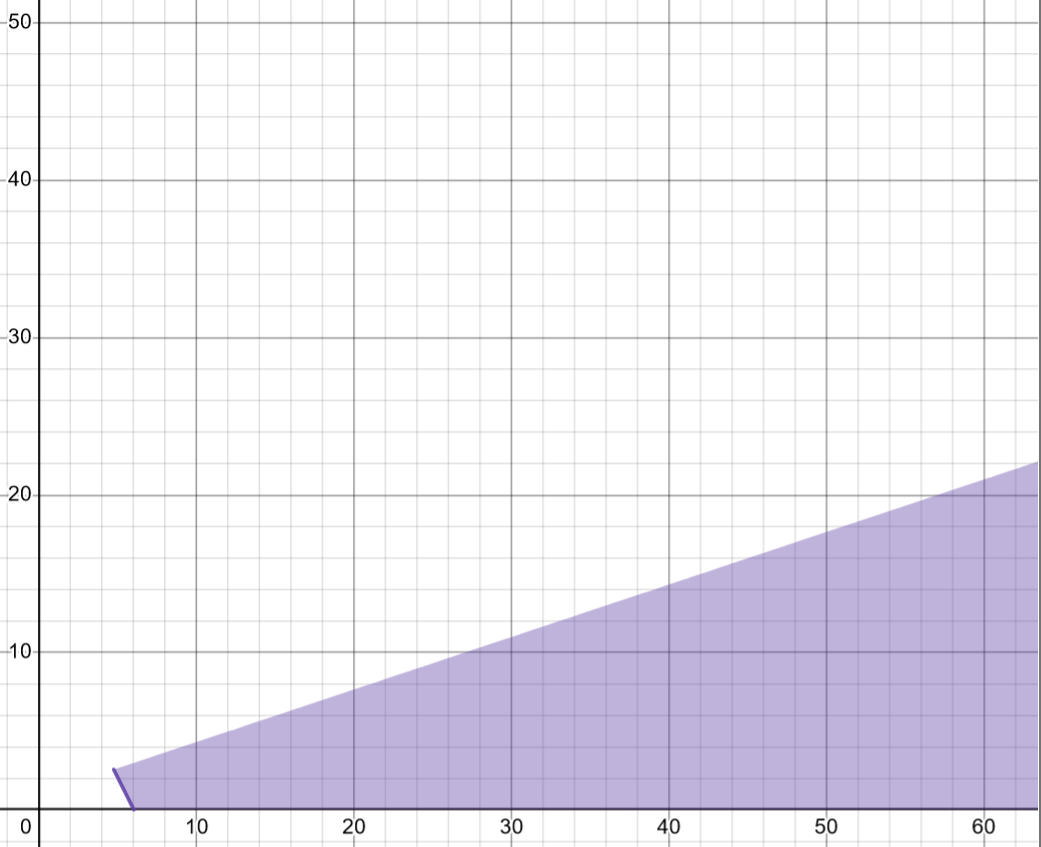
\includegraphics[scale = 0.8]{region1}
    \end{center}

    \item[(iii)]
    \begin{align*}
        \text{minimize} \:\:\: z = -x_1 - &x_2 \\
        \text{subject to} \:\:\:\: x_1 - 2x_2 &\geq 4 \\
        x_1 + x_2 &\leq 8\\
        x_1,x_2 &\geq 0\\
    \end{align*}
    \begin{center}
        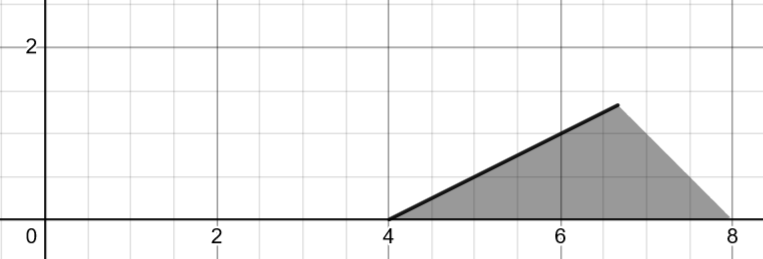
\includegraphics[scale = 0.8]{region2}
    \end{center}
    Since minima occur at critical values, we can see from the region above that the maximum occurs along the right edge boundary and the minimum value is $z = -8$.
\end{itemize}


\section*{Section 4.2 Problems}
\textbf{1.} Convert the following linear program to standard form:
\begin{align*}
    \text{maximize} \:\:\:\: z = 3x_1 + 5x_2 - &4x_3\\
    \text{subject to} \:\:\:\: 7x_1 - 2x_2 - 3x_3 &\geq 4\\
    -2x_1 + 4x_2 + 8x_3 &= -3\\
    5x_1 - 3x_2 - 2x_3 &\leq 9\\
    x_1 \geq 1, x_2 \leq 7, x_3 &\geq 0\\
\end{align*}
To begin, let us convert this problem to a minimization problem by multiplying $z$ by -1:
\[\hat{z} = -3x_1 - 5x_2 + 4x_3\]
From the constraint on $x_1$, let
\[x_1' = x_1 - 1\]
Then our first constraint becomes
\begin{align*}
    7(x_1' + 1) - 2x_2 - 3x_3 &\geq 4\\
    7x_1' + 7 - 2x_2 - 3x_3 &\geq 4\\
    7x_1' - 2x_2 - 3x_3 &\geq -3\\
    -7x_1' + 2x_2 + 3x_3 &\leq 3
\end{align*}
Introduce the slack variable $s_1 \geq 0$ so that
\[7x_1 + 2x_2' - 3x_3 + s_1 = 3\]
Now constraint 2 becomes
\begin{align*}
    -2(x_1' + 1) + 4x_2 + 8x_3 &= -3\\
    -2x_1' - 2  - 4x_2' + 8x_3 &= -3\\
    -2x_1' + 26 - 4x_2' + 8x_3 &= -3\\
    -2x_1' - 4x_2' + 8x_3 &= -29\\
    2x_1' + 4x_2' - 8x_3 &= 29\\
\end{align*}
Constraint 3 becomes
\begin{align*}
    5x_1 - 3x_2 - 2x_3 &= 5(x_1' + 1) - 3(7 - x_2') - 2x_3 \leq 9\\
    5x_1' + 5 - 21 + 3x_2' - 2x_3 &\leq 9\\
    5x_1' - 16 + 3x_2' - 2x_3 &\leq 9\\
    5x_1' + 3x_2' - 2x_3 &\leq 25\\
\end{align*}
Introduce the slack variable $s_2 \geq 0$ so that
\[5x_1' + 3x_2' - 2x_3 + s_2 = 25\]
Now $\hat{z}$ becomes
\begin{align*}
    \hat{z} &= -3(x_1' + 1) - 5(7 - x_2') + 4x_3 \\
    &= -3x_1' - 3 - 35 + 5x_2' + 4x_3 \\
    &= -3x_1' + 5x_2' + 4x_3 - 38
\end{align*}
Let $z' = \hat{z} + 38$ so that
\[z' = -3x_1' + 5x_2' + 4x_3\]
Then our problem in standard form takes the following form:
\begin{align*}
    \text{minimize} \:\:\:\: z' =&\: c^Tx \\
    \text{subject to} \:\:\:\: Ax &\geq 0\\
    x &\geq 0
\end{align*}
where $c = (-3,5,4,0,0)^T$, $x = (x_1', x_2', x_3, e_1, s_2)^T$, $b = (11, 29, 25)^T$,
\[A = \begin{pmatrix*}[r]
    7 & 2 & -3 & -1 & 0\\
    2 & 4 & -8 & 0 & 0\\
    5 & 3 & -2 & 0 & 1
\end{pmatrix*}\]

\textbf{2.} Convert the following linear program to standard form:
\begin{align*}
    \text{minimize} \:\:\:\: z = x_1 - 5x_2 - 7&x_3\\
    \text{subject to} \:\:\:\: 5x_1 - 2x_2 + 6x_3 &\geq 5\\
    3x_1 + 4x_2 - 9x_3 &= 3\\
    7x_1 + 3x_2 + 5x_3 &\leq 9\\
    x_1 \geq -2, x_2,x_3 & \text{ free.}
\end{align*}
For the constraint $x_1 \geq -2$, $x_1 + 2 \geq 0$, let $x_1' = x_1 + 2$, and since $x_2, x_3$ are free, let $x_2 = x_2' - x_2''$ and $x_3 = x_3' - x_3''$ where $x_2',x_2'', x_3',x_3'' \geq 0$. Then the first constraint becomes
\begin{align*}
    5x_1 - 2x_2 + 6x_3 &= 5(x_1' - 2) - 2(x_2' - x_2'') + 6(x_3' - x_3'') \geq 5\\
    5x_1' - 10 - 2x_2' + 2x_2'' + 6x_3' - 6x_3'' &\geq 5\\
    5x_1' - 2x_2' + 2x_2'' + 6x_3' - 6x_3'' &\geq 15
\end{align*}
Introduce the excess variable $e_1 \geq 0$ so that 
\[5x_1' - 2x_2' + 2x_2'' + 6x_3' - 6x_3'' - e_1 = 15\]
The second constraint becomes
\begin{align*}
    3(x_1' - 2) + 4(x_2' - x_2'') - 9(x_3'- x_3'') &= 3\\
    3x_1' - 6 + 4x_2' - 4x_2'' - 9x_3' + 9x_3'' &= 3\\
    3x_1' + 4x_2' - 4x_2'' - 9x_3' + 9x_3'' &= 9
\end{align*}
And the third constraint becomes
\begin{align*}
    7(x_1' - 2) + 3(x_2' - x_2'') + 5(x_3' - x_3'') &\leq 9\\
    7x_1' - 14 + 3x_2' - 3x_2'' + 5x_3' - 5x_3'' &\leq 9\\
    7x_1' + 3x_2' - 3x_2'' + 5x_3' - 5x_3'' &\leq 23
\end{align*}
Introduce the slack variable $s_2 \geq 0$ so that
\[7x_1' + 3x_2' - 3x_2'' + 5x_3' - 5x_3'' + s_2 = 23\]
Now, $z$ becomes
\begin{align*} 
    z &= x_1' - 2 - 5(x_2' - x_2'') - 7(x_3' - x_3'')\\
    &= x_1' - 5x_2' + 5x_2'' - 7x_3' + 7x_3'' - 2
\end{align*}
Let $z' = z + 2$ so that 
\[z' = x_1' - 5x_2' + 5x_2'' - 7x_3' + 7x_3''\]
So our problem becomes, in standard form,
\begin{align*}
    \text{minimize} \:\:\:\: z' = &c^Tx\\
    \text{subject to} \:\:\:\: Ax &\geq b\\
    x&\geq 0 
\end{align*}
where $c = (1, -5,5, -7, 7, 0, 0)^T$, $x = (x_1', x_2', x_2'', x_3', x_3'', e_1, s_2)^T$, $b = (15, 9, 23)^T$ and
\[A = \begin{pmatrix*}[r]
    5 & -2 & 2 & 6 & -6 & 1 & 0\\
    3 & 4 & -4 & -9 & 9 & 0 & 0\\
    7 & 3 & -3 & 5 & -5 & 0 & 1
\end{pmatrix*}\]

\section*{Section 4.3 Problems}
\textbf{1.} Consider the system of linear constraints
\begin{align*}
    2x_1 + x_2 &\leq 100\\
    x_1 + x_2 &\leq 80\\
    x_1 & \leq 40\\
    x_1,x_2 &\geq 0.
\end{align*}
\begin{itemize}
    \item[(i)] Write this system of constraints in standard form, and determine all the basic solutions (feasible and infeasible).
    \newline\newline
    Let $s_1,s_2,s_3 \geq 0$ be slack variables so that the system is in standard form:
    \begin{align*}
        2x_1 + x_2 + s_1 &= 100\\
        x_1 + x_2 + s_2 &= 80\\
        x_1 + s_3 &= 40 \\
        x_1,x_2,s_1,s_2,s_3 &\geq 0
    \end{align*}
    In matrix notation, we have
    \begin{align*}
        Ax &= b\\
        x &\geq 0\\
    \end{align*}
    where $x = (x_1,x_2,s_1,s_2,s_3)^T$, $b = (100,80,40)^T$, and
    \[A = \begin{pmatrix*}[r]
        2 & 1 & 1 & 0 & 0\\
        1 & 1 & 0 & 1 & 0 \\
        1 & 0 & 0 & 0 & 1
    \end{pmatrix*}\]
    Choosing the following bases to find all the basic solutions,
    \begin{align*}
        &1. \:\{x_1,x_2,s_1\} \:\:\: 2. \:\{x_1, x_2, s_2\} \:\:\: 3. \:\{x_1,x_2,s_3\}\\
        &4. \:\{x_1,s_1,s_2\} \:\:\: 5. \:\{x_1, s_1, s_3\} \:\:\: 6. \:\{x_1,s_2,s_3\}\\
        &7. \:\{x_2, s_1, s_2\} \:\:\: 8. \:\{x_2,s_1,s_3\} \:\:\: 9. \:\{x_2, s_2, s_3\}\\
        &10. \:\{s_1,s_2,s_3\}
    \end{align*}
    With these bases, we find the following basic solutions (notice that base 7 does not give a basic solution):
    \begin{center}
        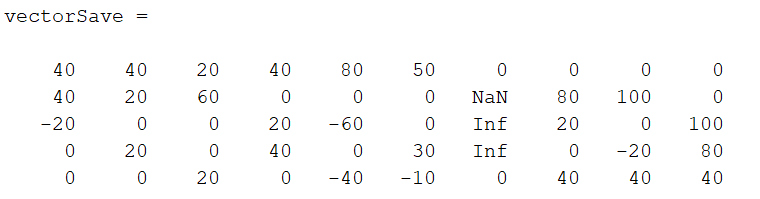
\includegraphics[scale = 0.8]{vectors}
    \end{center}
    Notice that bases 2, 3, 4, 8, and 10 give basic feasible solutions (since each element is greater than or equal to 0), whereas the other bases give infeasible solutions.

    \item[(ii)] Determine the extreme points of the feasible region (corresponding to both the standard form of the constraints, as well as the original version).
    \newline
    
    
    Since the extreme points on the region are given by the basic feasible solutions, we have that the following extreme points for the region in standard form:
    \begin{align*}
        x_a' = \begin{pmatrix}
            40\\
            20\\
            0\\
            20\\
            0
        \end{pmatrix}
        \:\:\:
       x_b' =  \begin{pmatrix}
            20\\
            60\\
            0\\
            0\\
            20
        \end{pmatrix}
        \:\:\:
       x_c' = \begin{pmatrix}
            40\\
            0\\
            20\\
            40\\
            0
        \end{pmatrix}
        \:\:\:
       x_d' = \begin{pmatrix}
            0\\
            80\\
            20\\
            0\\
            40
        \end{pmatrix}
        \:\:\:
       x_e' = \begin{pmatrix}
            0\\
            0\\
            100\\
            80\\
            40
        \end{pmatrix}
    \end{align*}        
    From these extreme points, we have the following extreme points of the original problem:
    \begin{align*}
        x_a = \begin{pmatrix}
            0\\
            0
        \end{pmatrix}
        x_b = \begin{pmatrix}
            40\\
            0
        \end{pmatrix}
        x_c = \begin{pmatrix}
            40\\
            20
        \end{pmatrix}
        x_d = \begin{pmatrix}
            20\\
            60
        \end{pmatrix}
        x_e = \begin{pmatrix}
            0\\
            80
        \end{pmatrix}
    \end{align*}
\end{itemize}

\textbf{4.} Consider the linear program
\begin{align*}
    \text{minimize} \:\:\: z = -5x_1 - 7x_2\\
    \text{subject to} \:\:\: -3x_1 + 2x_2 &\leq 30\\
    -2x_1 + x_2 &\leq 12\\
    x_1,x_2 &\geq 0.
\end{align*}
\begin{itemize}
    \item[(i)] Draw a graph of the feasible region.
        \begin{center}
            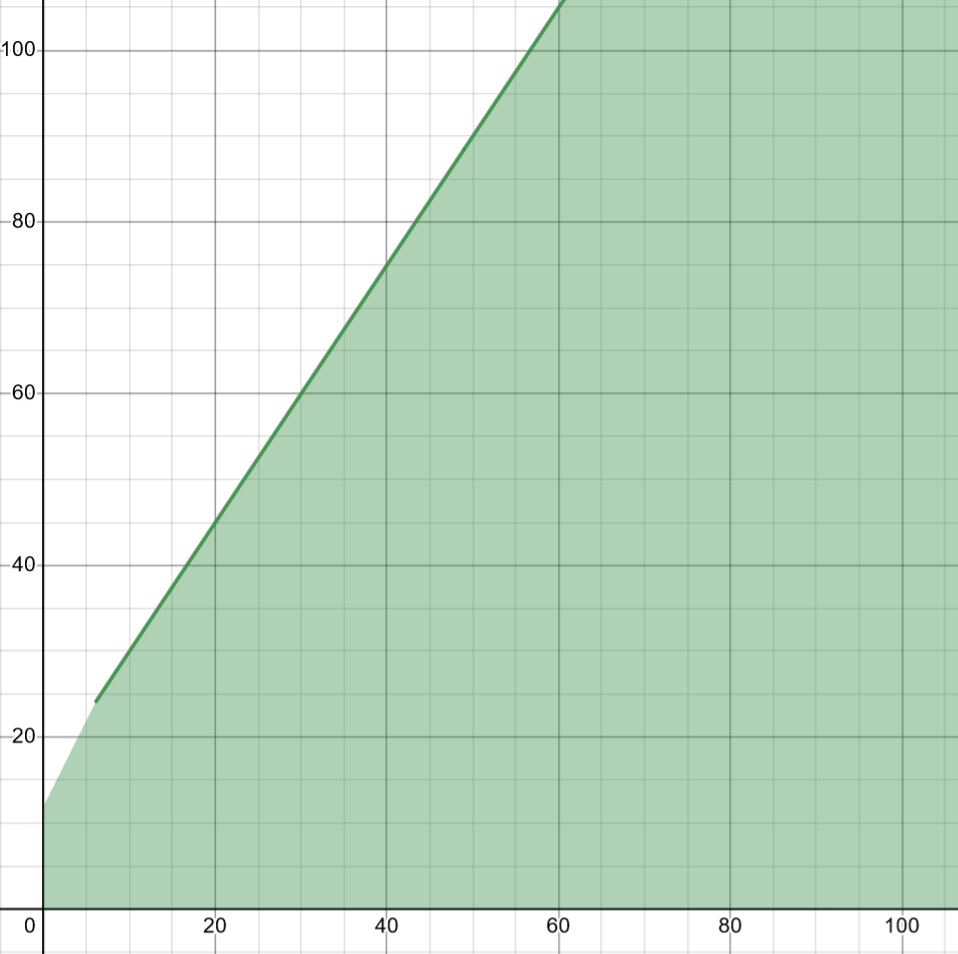
\includegraphics[scale = 0.8]{region3}
        \end{center}
    \item[(ii)] Determine the extreme points of the feasible region.
    \newline\newline
    From the plot in part (i), we can see that $(0,0)$ is an extreme point of the region. Further, solving when the constraints intersect, we find get that the solution of the linear system is also an extreme point:
    \begin{align*}
        -3x_1 + 2x_2 &= 30\\
        -2x_1 + x_2 &= 12
    \end{align*}
    which corresponds to the point $(6, 24)$. Further, finding when the constraints intersect the boundary $x_1 = 0$, we have that $(0,15)$ and $(0,12)$ are the intersection points, so $(0,12)$ is an extreme point, while $(0,15)$ lies outside of the feasible region.


    \item[(iii)] Determine two linearly independent directions of unboundedness.
    \newline\newline
    From the figure above, we can see that $(1,0)^T$ is a direction of unboundedness, and from the constraint $-3x_1 + 2x_2 \leq 30$ we can see that $(3,2)^T$ is also a direction of unboundedness.

    \item[(iv)] Convert the linear program to standard form and determine the basic feasible solutions and two linearly independent directions of unboundedness for this version of the problem. Verify that the directions of unboundedness satisfy $Ad = 0$ and $d \geq 0$.
    \newline\newline
    Converting to standard form, add a slack variable $s_1 \geq 0$ to the first constraint, and a slack variable $s_2 \geq 0$ to the second constraint so that our linear program takes the following form:
    \begin{align*}
        \text{minimize} \:\:\:\: z =& \:c^Tx\\
        \text{subject to} \:\:\:\: Ax &= b\\
        x &\geq 0\\
    \end{align*}
    where $c = (-5,-7,0,0)^T$, $x = (x_1,x_2,s_1,s_2)^T$, $b = (30,12)^T$, and
    \[A = \begin{pmatrix*}[r]
        -3 & 2 & 1 & 0\\
        -2 & 1 & 0 & 1
    \end{pmatrix*}\]
    Using the script to find the basic solutions, we find the following:
    \begin{center}
        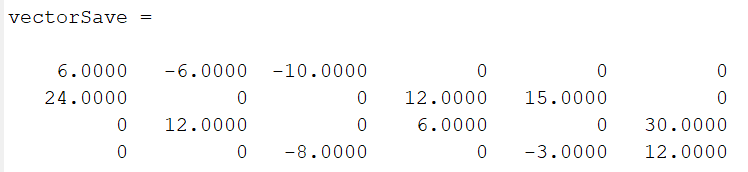
\includegraphics[scale = 0.75]{vector43}
    \end{center}
    From this we can see the basic feasible solutions are as follows:
    \begin{align*}
        x_a' = \begin{pmatrix*}[r]
            6\\
            24\\
            0\\
            0
        \end{pmatrix*}
        \:\:\:
        x_b' = \begin{pmatrix}
            0\\
            12\\
            6\\
            0
        \end{pmatrix}
        \:\:\:
        x_c' = \begin{pmatrix}
            0\\
            0\\
            30\\
            12
        \end{pmatrix}
    \end{align*}    
    
\end{itemize}



\textbf{6.} Consider the system of constraints
\begin{align*}
    2x_1 + x_2 &\leq 3\\
    3x_1 + x_2 &\leq 4\\
    4x_1 + x_2 &\leq 5\\
    5x_1 + x_2 &\leq 6\\
    x_1,x_2 &\geq 0
\end{align*}
\begin{itemize}
    \item[(i)] Determine the extreme points for the feasible region.
    \newline\newline
    From the above constraints, we can see that that the boundaries of the first four constraints intersect at the point $(1,1)^T$ and that the constraints $x_1, x_2 \geq 0$ intersect at $(0,0)^T$. Now we wish to find when the first four constraints intersect the last two and which of those intersection points is inside the feasible region. Let us begin by seeing when the first four constraints intersect the boundary $(x_1 = 0)$.
    \begin{align*}
        x_2 &= 3\\
        x_2 &= 4\\
        x_2 &= 5\\
        x_2 &= 6
    \end{align*}
    From these intersection points, we see that the point $(0,3)$ is within the feasible region. Now let us inspect the constraints on the boundary $(x_2 = 0)$:
    \begin{align*}
        2x_1 &= 3\\
        3x_1 &= 4\\
        4x_1 &= 5\\
        5x_1 &= 6
    \end{align*}
    From this we can see the intersection point $(6/5, 0)$ is within the feasible region. Thus, our critical points of the feasible region are
    \begin{align*}
        x_a = \begin{pmatrix}
            0\\
            0
        \end{pmatrix}
        ,\:\:\:\:
        x_b = \begin{pmatrix}
            1\\
            1
        \end{pmatrix}
        ,\:\:\:\:
        x_c = \begin{pmatrix}
            0\\
            3
        \end{pmatrix}
        ,\:\:\:\:
        x_d = \begin{pmatrix}
            6/5\\
            0
        \end{pmatrix}
    \end{align*}

    \item[(ii)] Convert the problem to standard form, and determine the basic feasible solutions.
    \newline\newline
    Converting the problem to standard form, we have the following system:
    \begin{align*}
        Ax &= b\\
        x &\geq 0\\
    \end{align*}
    where $x = (x_1, x_2, s_1, s_2, s_3, s_4)^T$, $b = (3, 4, 5, 6)^T$, and 
    \[A = \begin{pmatrix}
        2 & 1 & 1 & 0 & 0 & 0\\
        3 & 1 & 0 & 1 & 0 & 0\\
        4 & 1 & 0 & 0 & 1 & 0\\
        5 & 1 & 0 & 0 & 0 & 1
    \end{pmatrix}\]
    Writing a small script (similar to the last couple problems), we find, in the following figure, the following basic solutions:
    \begin{center}
        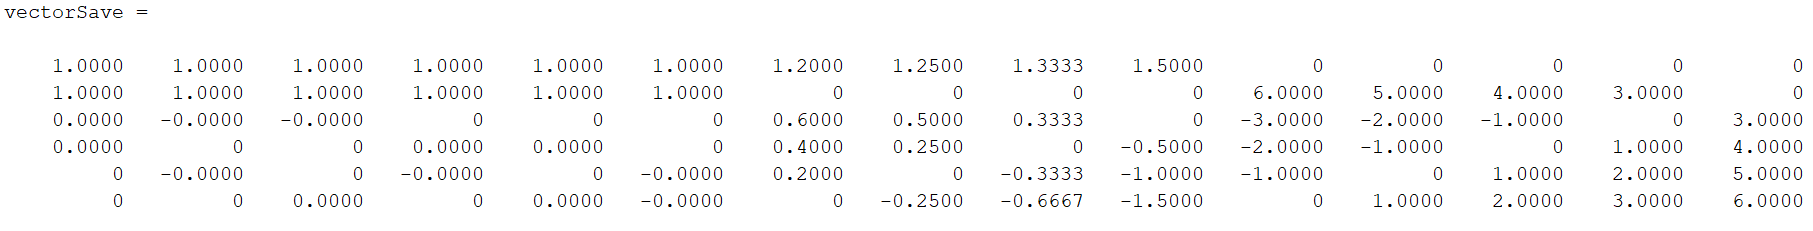
\includegraphics[scale = 0.5]{15vectors}
    \end{center}
    From these basic solutions, we find the following basic feasible solutions:
    \begin{align*}
        x_a' = \begin{pmatrix}
            1\\
            1\\
            0\\
            0\\
            0\\
            0
        \end{pmatrix}
        ,\:\:\:
        x_b' = \begin{pmatrix}
            6/5\\
            0\\
            3/5\\
            2/5\\
            1/5\\
            0
        \end{pmatrix}
        ,\:\:\:
        x_c' = \begin{pmatrix}
            0\\
            3\\
            0\\
            1\\
            2\\
            3
        \end{pmatrix}
        ,\:\:\:
        x_d' = \begin{pmatrix}
            0\\
            0\\
            3\\
            4\\
            5\\
            6
        \end{pmatrix}       
    \end{align*}

    \item[(iii)] Which basic feasible solution corresponds to the extreme point $(1,1)^T$? How many different bases can be used to generate this basic feasible solution? Which of these bases are adjacent?
    \newline\newline
    Notice from above that the basic feasible solution $(1,1,0,0,0,0)^T$ corresponds to the extreme point $(1,1)^T$. From the table above, we can see six bases can be used to generate this basic solution. Call these bases
    \[b_1 = \begin{pmatrix}
        x_1\\
        x_2\\
        s_1\\
        s_2
    \end{pmatrix}
    ,\:\:\:
    b_2 = \begin{pmatrix}
        x_1\\
        x_2\\
        s_1\\
        s_3
    \end{pmatrix}
    ,\:\:\:
    b_3 = \begin{pmatrix}
        x_1\\
        x_2\\
        s_1\\
        s_4
    \end{pmatrix}
    ,\:\:\:
    b_4 = \begin{pmatrix}
        x_1\\
        x_2\\
        s_2\\
        s_3
    \end{pmatrix}
    ,\:\:\:
    b_5 = \begin{pmatrix}
        x_1\\
        x_2\\
        s_2\\
        s_4
    \end{pmatrix}
    ,\:\:\:
    b_6 = \begin{pmatrix}
        x_1\\
        x_2\\
        s_3\\
        s_4
    \end{pmatrix}
    \]
    From the above table, we can see the following bases are adjacent:
    \begin{align*}
        &b_1 \:\: \& \:\: b_2 \\
        &b_1 \:\: \& \:\: b_3 \\
        &b_1 \:\: \& \:\: b_4 \\
        &b_1 \:\: \& \:\: b_5 \\
        &b_2 \:\: \& \:\: b_3 \\
        &b_2 \:\: \& \:\: b_4 \\
        &b_2 \:\: \& \:\: b_6 \\
        &b_3 \:\: \& \:\: b_5 \\
        &b_3 \:\: \& \:\: b_6 \\
        &b_4 \:\: \& \:\: b_5 \\
        &b_4 \:\: \& \:\: b_6 \\
        &b_5 \:\: \& \:\: b_6 \\
    \end{align*}
\end{itemize}

\textbf{13.} Suppose that a linear program includes a free variable $x_i$. In converting this problem to standard form, $x_i$ is replaced by a pair of nonnegative variables:
\[x_i = x_i' - x_i'', \:\:\:\: x_i', x_i'' \geq 0.\]
Prove that no basic feasible solution can include both $x_i'$ and $x_i''$ as basic variables.
\newline\newline
Proof: Let $A$ be the constraint matrix for the linear program before it is converted into standard form and let $\vec{a}_i$ be the $i^{\text{th}}$ column of $A$ corresponding to the variable $x_i$ and express how $x_i$ appears in the constraint matrix $A$ by
\[\vec{a}_i x_i = \begin{pmatrix}
    a_{1i}\\
    a_{2i}\\
    \vdots\\
    a_{mi}\\
\end{pmatrix}x_i\]
For this proof, call the above vector the \say{constraint vector}. Now suppose in converting the linear program to standard form, $x_i$ is replaced by $x_i'$ and $x_i''$ such that
\[x_i = x_i' - x_i'', \:\:\: x_i', x_i'' \geq 0\]
Denote the constraint matrix of the linear program in standard form by $A_s$. The constraint vector for $x_i$ becomes
\begin{align*}
    \vec{a}_ix_i &= \vec{a}_i(x_i' - x_i'') \\
    &= \vec{a}_ix_i' - \vec{a}_ix_i''
\end{align*}
Let $\vec{a}_i' = \vec{a}_i$ and $\vec{a}_i'' = -\vec{a}_i$ be the constraint vectors corresponding to $x_i'$ and $x_i''$, respectively. Notice that $\vec{a}_i'$ and $\vec{a}_i''$ are linearly dependent, since $\vec{a}_i' = -\vec{a}_i''$. That is, for any basis including both $x_i'$ and $x_i''$, we have that the submatrix of $A_s$ corresponding to this basis will have at least one linearly dependent column, which means that any basis including $x_i'$ and $x_i''$ will not give a basic solution.


\section*{Section 4.4 Problems}
\textbf{2.} Let $x$ be an element of a convex set $S$. Assume that $x_1 = x + \epsilon_1p \in S$ and $x_2 = x - \epsilon_2p \in S$ where $p \neq 0$ and $\epsilon_1,\epsilon_2 > 0$. Prove that $x$ is a convex combination of $x_1$ and $x_2$. That is, prove that 
\[x = \alpha x_1 + (1 - \alpha)x_2\]
where $0 < \alpha < 1$, and determine the value of $\alpha$.
\newline\newline
Proof: Let $x \in S$ where $S$ is a convex set and assume that $x_1 = x + \epsilon_1 p \in S$ and $x_2 = x - \epsilon_2p \in S$ where $p \neq 0$. Solving these relationships for $x$, we have
\begin{align*}
    x &= x_1 - \epsilon_1p\\
    x &= x_2 + \epsilon_2p
\end{align*}
Multiplying the first equation above by $\epsilon_2/\epsilon_1$ and adding to the first equation, we find
\[\left(1 + \frac{\epsilon_2}{\epsilon_1}\right)x = \frac{\epsilon_2}{\epsilon_1}x_1 + x_2\]
Dividing, we find
\[x = \frac{\epsilon_2}{\epsilon_1 + \epsilon_2}x_1 + \frac{\epsilon_1}{\epsilon_1 + \epsilon_2}x_2\]
Let $\alpha = \epsilon_2/(\epsilon_1 + \epsilon_2)$ and notice
\begin{align*}
    1 - \alpha &= 1 - \frac{\epsilon_2}{\epsilon_1 + \epsilon_2} \\
    &= \frac{\epsilon_1 + \epsilon_2 - \epsilon_2}{\epsilon_1 + \epsilon_2}\\
    &= \frac{\epsilon_1}{\epsilon_1 + \epsilon_2}
\end{align*}
Then we have 
\[x = \alpha x_1 + (1- \alpha)x_2\]
Further notice that $\epsilon_1 + \epsilon_2 > \epsilon_2$, so $0 < \alpha < 1$.
\newline\newline



\textbf{6.} Consider the linear program
\begin{align*}
    \text{minimize} \:\:\: z = 2x_1 - &3x_2\\
    \text{subject to} \:\:\: 4x_1 + 3x_2 &\leq 12\\
    x_1 - 2x_2 &\leq 2\\
    x_1, x_2 &\geq 0.
\end{align*}
Represent the point $x = (1,1)^T$ as a convex combination of extreme points plus, if applicable, a direction of unboundedness. Find three different representations.
\newline\newline
Solving for when all the constraints intersect, we find the following extreme points:
\[x_a = \begin{pmatrix}
    0\\
    0
\end{pmatrix}
,\:\:\:
x_b = \begin{pmatrix}
    0\\
    4
\end{pmatrix}
,\:\:\:
x_c = \begin{pmatrix}
    2\\
    0
\end{pmatrix}
,\:\:\:
x_d = \begin{pmatrix}
    30/11\\
    4/11
\end{pmatrix}
\]
Consider the direction $p = (1,1)^T$ and notice that $x_{p_1} = x + 5/4p = (9/4,1)^T$ and $x_{p_2} = x - p = (0,1)^T$ lie on the boundary of the feasible region. Notice that 
\begin{align*}
    \frac{1}{4}x_b + \frac{3}{4}x_a &= (0,1)^T + (0,0)^T\\
    &= (0,1)^T\\
    &= x_{p_1}
\end{align*}
So $x_{p_1} = \alpha_1x_b + \alpha_2x_a$ where $\alpha_1 = 1/4$ and $\alpha_2 = 3/4$. Also notice
\begin{align*}
    \frac{33}{40}x_d + \frac{7}{40}x_b &= (9/4, 3/10)^T + (0, 7/10)^T\\
    &= (9/4, 1)^T
\end{align*}
So $x_{p_2} = \alpha_3x_d + \alpha_4x_b$ where $\alpha_3 = 33/40$ and $\alpha_4 = 7/40$. Also notice that
\begin{align*}
    x &= \frac{5}{9}x_{p_1} + \frac{4}{9}x_{p_2}\\
    &= (1,4/9)^T + (0,5/9)^T\\
    &= (1,1)^T
\end{align*}
Finally, from above, we have
\begin{align*}
    x &= \frac{5}{9}\left[\frac{33}{40}\begin{pmatrix}
        30/11\\
        4/11
    \end{pmatrix} + \frac{7}{40}\begin{pmatrix}
        0\\
        4
    \end{pmatrix}
    \right] + \frac{4}{9}\left[\frac{1}{4}\begin{pmatrix}
        0\\
        4
    \end{pmatrix} + \frac{3}{4}\begin{pmatrix}
        0\\
        0
    \end{pmatrix} \right] \\
    &= \frac{33}{72}x_d + \frac{7}{72}x_b + \frac{8}{72}x_b + \frac{24}{72}x_a\\
    &= \frac{24}{72}x_a + \frac{15}{72}x_b + \frac{33}{72}x_d\\
\end{align*}
So we have that $x$ is a convex combination of the extreme points.

\end{document}
